En este capítulo, se detalla el diseño e implementación del sistema. Tecnologías utilizadas, arquitectura
y diseño, así como, detalles de implementación y patrones que se han seguido.

\section{Tecnologías}

Este proyecto ha sido desarrollado empleando diversas tecnologías y soluciones de $Python$.

$Python$\footnote{\url{https://www.python.org/}} es un lenguaje multiparadigma que es ampliamente utilizado en ámbitos científicos y de investigación.
Cuenta con multitud de herramientas para la realización de $tests$, gestión de dependencias, etc., entre las
que se encuentran $Unittest$\footnote{\url{https://docs.python.org/3/library/unittest.html}} (tests unitarios) y $Pip$\footnote{\url{https://pypi.python.org/pypi/pip}} (gestor de dependencias), que han sido empleadas en este trabajo.

Se ha optado por utilizar el lenguaje de programación $Python$, en su versión 3, concretamente, en el momento de la realización de este trabajo el desarrollo se ha realizado
bajo la versión 3.6.2 de dicho lenguaje.

La implementación de $Python$ utilizada es $CPython$\footnote{\url{https://www.toptal.com/python/por-que-hay-tantos-pythons/es}}.

Además, se han empleado los siguientes paquetes:

\begin{itemize}
  \item \textit{NumPy} como librería fundamental para computación científica del ecosistema \textit{SciPy}.
  \item \textit{Matplotlib} como librería para creación de gráficas del ecosistema \textit{SciPy}.
  \item \textit{Plotly} como librería gráfica, utilizada en este caso sólo para representar figuras en tres dimensiones.
\end{itemize}

Por último, para su desarrollo, se han utilizado otras herramientas como: \textit{Git} y \textit{Git-flow}, \textit{Github},
\textit{Travis}, \textit{Landscape}, \textit{Coveralls} y \textit{Docker}.

\section{Arquitectura y diseño}

Para el desarrollo de este proyecto se ha optado por seguir dos paradigmas simultáneamente. Por un lado,
se ha seguido el paradigma orientado a objeto, esto es, modelizar las partes del sistema con objetos que encapsulan
las propiedades y métodos necesarios según las necesidades u objetivos de cada una de ellas y, las cuales,
se describen en la siguiente sección de este capítulo. Por otro lado, se ha seguido el paradigma funcional, esto es,
diseñar el sistema, o partes de él, en forma de funciones, las cuales para ejecutar su lógica utilizan únicamente
los parámetros que recibe.

\begin{figure}[h]
\centering
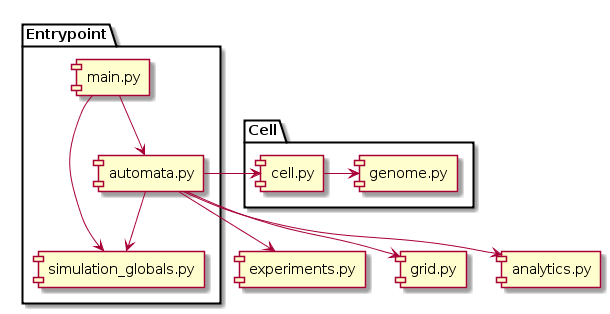
\includegraphics[scale=0.8]{figures/architecture}
\caption{Diagrama de componentes del sistema.}
\label{fig:arch}
\end{figure}

Ambos paradigmas, comentado brevemente en el párrafo anterior, tienen muchos más aspectos, enfoques y soluciones
de las que se comentan. El programa cuenta con un único punto de entrada, como se muestra en la figura ~\ref{fig:arch},
en este caso, siguiendo el patrón
\textit{Singleton}. En cuanto a los patrones utilizados, se van a describir en la siguiente sección de este
capítulo donde se presentan los diferentes módulos del mismo.

\section{Módulos del sistema}

En este caso, se han implementado $6$ módulos~\ref{fig:arch}. El módulo principal, \textit{automata.py}, presenta
una clase que sigue el patrón \textit{Estrategia} y, el cual, engloba la función principal de ejecución,
así como, el resto de funciones necesarias para su correcta ejecución. Además, importa y utiliza
el resto de módulos, los caules, se describen a continuación.

\subsection{Módulo \textit{genome.py}}

Este es el primero de los módulos que se ha desarrollado, y es el más simple de todos. Consta de
una clase que contiene únicamente cinco variables binarias, una por cada mutación que se
modeliza en este sistema.

Como se ha descrito previamente, las mutaciones que contiene esta clase son las siguientes:

\begin{itemize}
    \item \textbf{SG}: Autogeneración de los mensajes de crecimiento. Esto es, la mutación que permite que la
    célula genere sus propios mensajes para ejecutar la división con independencia externa.
    \item \textbf{IGI}: Inhibición de las señales de anticrecimiento. Esto es, ante la recepción de una orden
    de detener su crecimiento, la célula tiene una mutación que le permite un mecanismo de ignorancia de los mismos.
    \item \textbf{EA}: Evasión de apoptosis. Esto es, la célula puede, mediante mutación, no hacer caso ante
    una orden de apoptosis, o muerte celular controlada.
    \item \textbf{EI}: Inmortalidad efectiva. Esto es, la célula adquiere una mutación que permite evitar un límite
    replicativo existente, entre otros factores, por el tamaño del telómero.
    \item \textbf{GI}: Inestabilidad genética. Esto es, una mutación que permite a la célula acumular más daño genético, es decir,
    la tasa de mutación base se va incrementando con el paso del tiempo.
\end{itemize}

Además, expone un método que permite obtener el número de mutaciones que tiene cada instancia
de este tipo.

En definitiva, se trata de una clase que, por composición, estará contenida dentro de otra clase
que modeliza a la célula, representando su genoma, y que se explica a continuación.

\subsection{Módulo \textit{cell.py}}

El siguiente módulo, partiendo de la clase genoma, es el que contiene la clase que modeliza
a cada una de las células de la simulación.

Como se ha comentado previamente contiene, por composición, un atributo que representa
al genoma de la célula y que se trata de un objeto tal y como se ha descrito en la sección anterior de este capítulo.
Además, presenta algunos atributos más necesarios para la simulación, y son:

\begin{itemize}
    \item Atributo que representa el tamaño del telómero.
    \item Atributo que representa la tasa de mutación de la célula.
    \item Atributo que representa su posición en la rejilla, es decir, un conjunto de tres elementos
    que representan su posición en cada una de las dimensiones ($(x,y,z)$).
\end{itemize}

Por último, cuenta con varios métodos necesarios para la simulación, y son los siguientes:

\begin{itemize}
    \item \textit{decrease\_telomer()}: Método que se encarga de cambiar el estado interno del objeto, realizando un decrecimiento en una unidad del telómero.
    \item \textit{increment\_base\_muration\_rate(i)}: Las células ven alterada su tasa de mutación base, utilizada para originar nuevas mutaciones durante la mitosis,
    con la presencia de la mutación asociada a la inestabilidad genética o $GI$. Este método realiza este proceso de acuerdo a una tasa de modificación, o incremento,
    de esta tasa, la cual es recibida por parámetros.
    \item \textit{mutations()}: Método que devuelve el número de mutaciones que tiene la célula en su genoma.
    \item \textit{add\_mutations()}: Método que se encarga de generar las nuevas mutaciones que pueden tener lugar durante la mitosis.
    \item \textit{perform\_mitosis()}: El proceso de mitosis queda modelado en este método, esto es, incrementar tasa de mutación base, añadir nuevas mutaciones y
    realizar una copia de sí misma.
\end{itemize}

\subsection{Módulo \textit{simulation\_globals.py}}

De cara a realizar la simulación son necesarios una serie de parámetros que se necesitarán manipular
para realizar los experimentos que se describirán en capítulos posteriores. Esto lleva al siguiente módulo,
en el cual se tiene una clase que contiene sólo atributos que almacenan todos estos parámetros.

Dichos parámetros son los siguientes:

\begin{itemize}
    \item Tasa de mutación base o \textit{m}.
    \item Tamaño del telómero o \textit{tl}.
    \item Probabilidad de evasión de apoptosis o \textit{e}.
    \item Factor de incremento de la tasa de mutación base o \textit{i}.
    \item Probabilidad de matar a un vecino para realizar la mitosis o \textit{g}.
    \item Probabilidad de muerte aleatoria de la célula o \textit{a}.
    \item Límite espacial predefinido.
    \item Límite inferior para evento mitótico en el futuro.
    \item Límite superior para evento mitótico en el futuro.
\end{itemize}

En este fichero, además, se encuentran los valores por defecto de la simulación según los autores
del artículo \cite{jsantos-amonteagudo-1-2014} en el que se basa este trabajo. En este caso,
se declaran como constantes, ya que estos, en caso de ser utilizados en la simulación, no varían.

\subsection{Módulo \textit{experiments.py}}

Para realizar la mitosis, se necesitan realizar varias pruebas o experimentos. Estos
están contenidos dentro de una clase como métodos. Los parámetros necesarios para ejecutar dichas
pruebas se reciben por parámetros. Los métodos, son los siguientes:

\begin{itemize}
  \item \textit{random\_death\_test()}: Prueba que indica si hay o no muerte aleatoria de la célula.
  \item \textit{random\_death\_test(n, ea)}: Prueba que indica si hay muerte por daño genético según
  el número de mutaciones de la célula que está realizando el proceso de mitosis, excepto que esté
  presente el marcador con la mutación que permite evadir la apoptosis.
  \item \textit{random\_death\_test(sg, spatial\_boundary)}: Prueba que está dentro del
  límite espacial o, lo que es lo mismo, si existe suficiente factor de crecimiento como
  para ejecutar la mitosis. Excepto, si tiene presente el marcador $sg$, que permite
  ejecutar la mitosis si la célula se encuentra fuera de dicho espacio.
  \item \textit{random\_death\_test(igi)}: Prueba que comprueba si existe espacio para ubicar la célula
  hija una vez realizada la mitosis. Si no hay espacio y la célula tiene la mutación asociada al
  marcador $igi$, podrá matar a un vecino para ubicar a la célula hija.
  \item \textit{random\_death\_test(tl, ei)}: Prueba que comprueba si el telómero tiene tamaño
  mayor a $0$ para realizar la mitosis. Si el tamaño es $0$, la célula puede realizar mitosis
  si tiene presente la mutación asociada al marcador $ei$.
\end{itemize}

\subsection{Módulo \textit{grid.py}}

El módulo \textit{grid.py} almacena la información relativa a la rejilla en la que tiene lugar
la simulación. Esto es, tiene como propiedad o atributos el ancho, alto y largo del mismo.

Pero, la parte útil de este módulo son los métodos que permiten a la simulación obtener el vecindario,
controlando sus límites, y obtener qué celdas del vecindario están ocupadas y cuales no. Por tanto,
sus métodos son los siguientes:

\begin{itemize}
  \item \textit{neighborhood(origin, radio)}: Método que recibe un centro de tipo $(x,y,z)$ y un radio, para devolver una lista con las posiciones
  que conforman el vecindario.
  \item \textit{filter(value, limit)}: Método que permite saber si un valor está dentro de un límite espacial. Es utilizada en únicamente en el siguiente métodos.
  \item \textit{check\_limits(cube, limit)}: Método que comprueba que, de una lista de posiciones que conforman el vecindario, no existe una posición que exceda el
  límite de la rejilla. Devuelve, la lista sin dichas posiciones.
  \item \textit{classify\_neighborhood(cube, cells)}: Métdodo que clasifica las células de un cubo que representa un vecindario en función de las posiciones
  ocupadas y las que están libres.
\end{itemize}

\subsection{Módulo \textit{automata.py}}

Módulo principal del sistema que contiene la lógica de ejecución del mismo~\ref{fig:automata}. El sistema
está diseñado siguiendo el patrón \textit{Singleton}, es decir, sólo hay un objeto
autómata que, implementando el patrón \textit{estrategia}, tiene un, método con
la lógica de ejecución.

La lógica de ejecución se encuentra descrita en la sección 4.8 de este documento.

Además, tiene como atributos la agenda de eventos mitóticos, así como, el objeto que
encapsula los experimentos necesarios para saber si se aplica o no mitosis a cada célula, los
parámetros de simulación, el objeto con la lógica necesaria para gestionar la rejilla y, por último,
la responsabilidad de generar las medidas utilizando el módulo de analítica que se describe a continuación.

\begin{figure}[h]
\centering
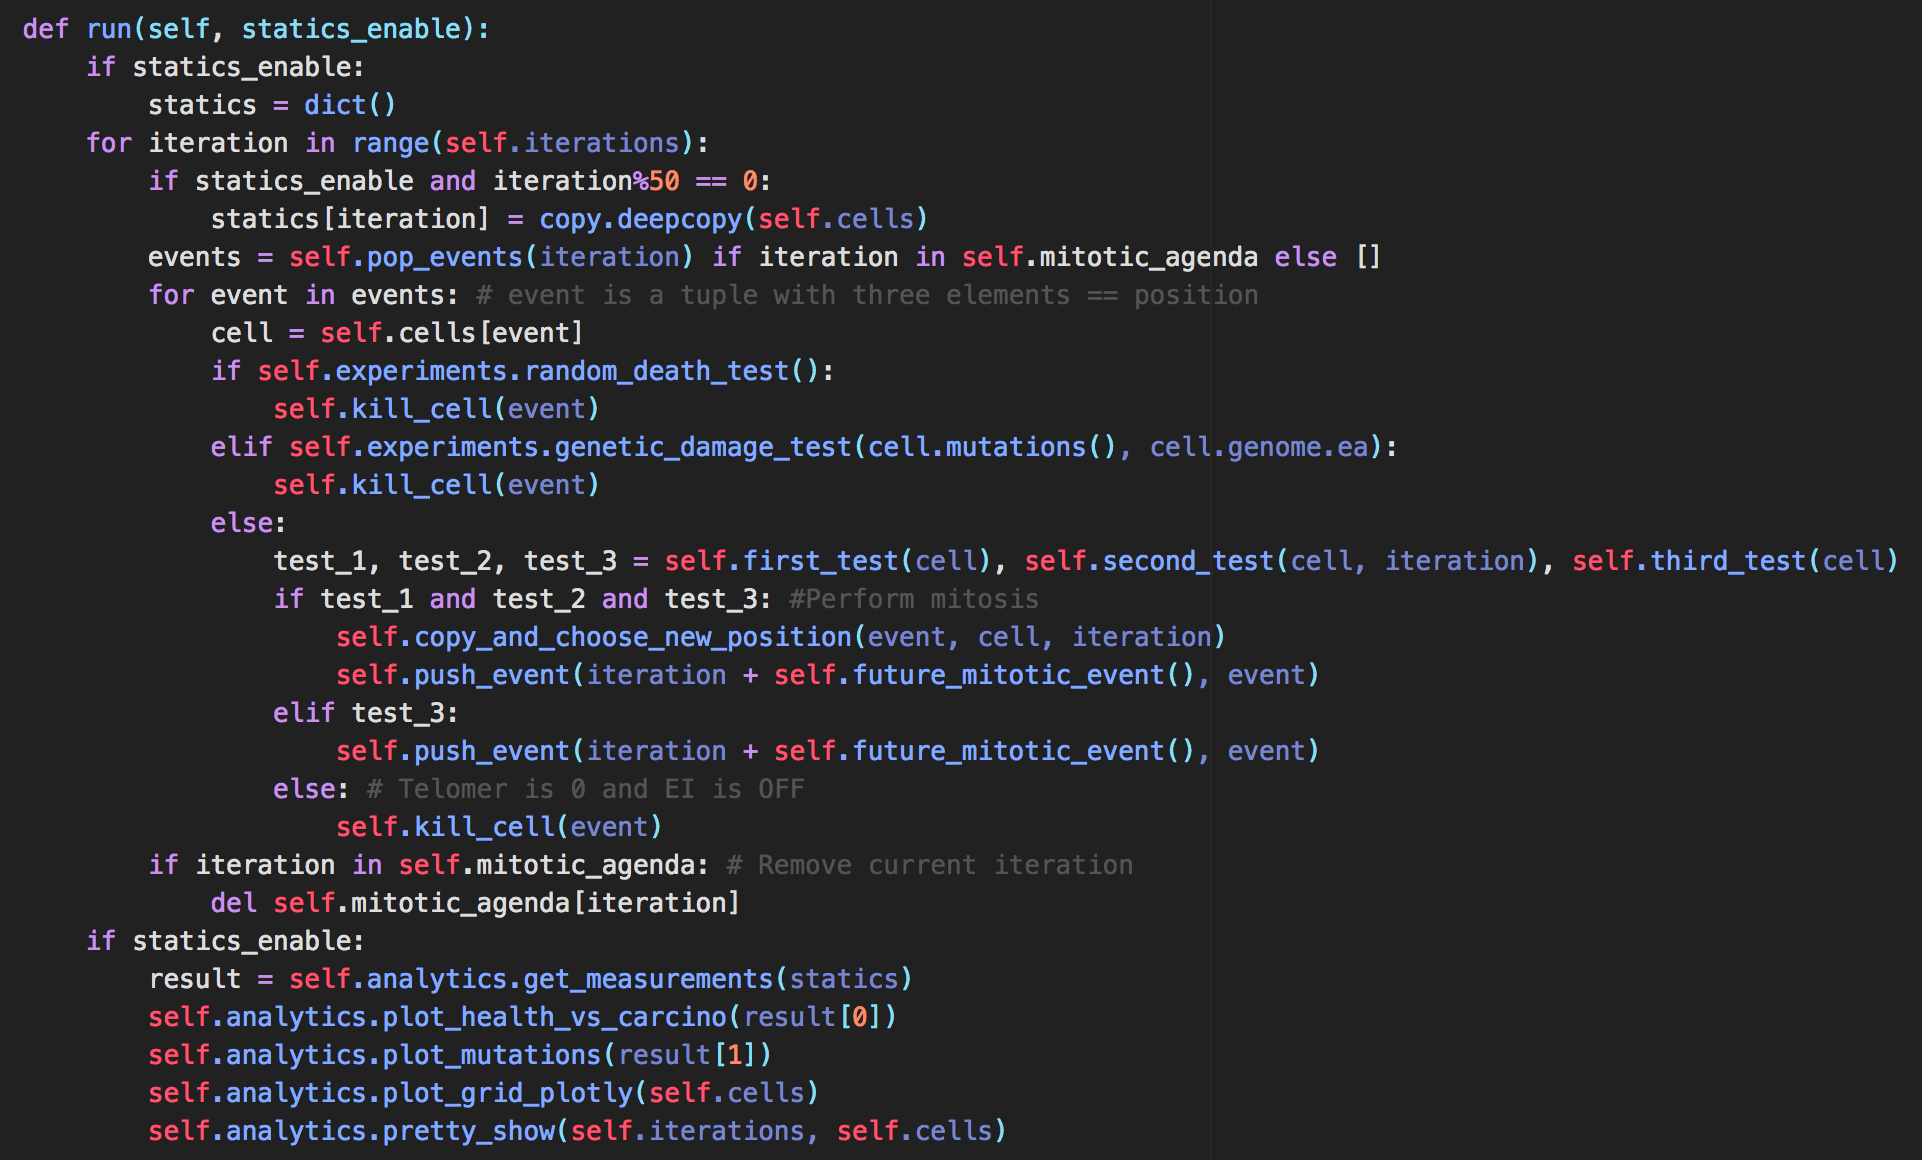
\includegraphics[scale=0.45]{figures/alg}
\caption{Código con el bucle principal de la simulación.}
\label{fig:automata}
\end{figure}

\subsection{Módulo \textit{analytics.py}}

Este último módulo, reúne las funciones necesarias para hacer medidas sobre las células
de la rejilla, como por ejemplo, células sanas o cancerígenas, cuántas células tienen un
determinado marcador del cáncer activo, etc.

Además, contiene funciones para construir y mostrar gráficas con vista a presentar la evolución
del sistema a lo largo de la simulación.

\section{Instalación y ejecución}

En esta última sección del capítulo dedicado a la implementación, se expone la información necesaria
para su instalación y uso. Existen dos formas de conseguirlo, la primera, a través de una ejecución
nativa, es decir, sobre la propia máquina local. En segundo lugar, sobre \textit{Docker}, lo cual permite
no realizar ninguna instalación sobre la máquina local.

\subsection{Prerrequisitos}

Dependiendo del tipo de instalación, se dan los siguientes prerrequisitos:

\begin{itemize}
  \item Para una ejecución sobre la máquina local, se necesita:
        \item Instalar la versión 3.6+ de \textit{Python}\footnote{\url{https://www.python.org/downloads/}}.
        \item Instalar el gestor de paquetes de \textit{Python}, \textit{pip}\footnote{\url{https://pip.pypa.io/en/stable/installing/}}.
        \item Instalar el control de versiones \textit{Git}\footnote{\url{https://git-scm.com/book/en/v2/Getting-Started-Installing-Git}}.
        \item Clonar el repositorio ejecutando en consola \textit{git clone \url{https://github.com/MULCIA/TFMSTGCA.git}}.
        \item Instalar dependencias con \textit{pip}, para ello, ejecutar en consola \textit{pip install -r requirements.txt}.
  \item Para una ejecución con \textit{Docker} se necesita:
        \item Instalar la última versión de \textit{Docker}\footnote{\url{https://docs.docker.com/engine/installation/}}.
        \item Instalar el control de versiones \textit{Git}\footnote{\url{https://git-scm.com/book/en/v2/Getting-Started-Installing-Git}}.
        \item Clonar el repositorio ejecutando en consola \textit{git clone \url{https://github.com/MULCIA/TFMSTGCA.git}}.
\end{itemize}

\subsection{Ejecución}

Dependiendo del modo elegido, es decir, ejecución en máquina local o ejecución en \textit{Docker}, su ejecución es diferente.

En primer lugar, se describe como hacer una ejecución en máquina local. Una vez cumplidos los requisitos descritos anteriormentes,
para ejecutar el proyecto sólo hay que ejecutar, dentro del directorio que contiene el proyecto, el siguiente comando:
\textit{python main.py}.

Su ejecución se realiza automáticamente y al finalizar mostrará una serie de gráficas:

\begin{itemize}
  \item Gráfica que muestra la evolución en número de las células sanas frente a las células cancerosas.
  \item Gráfica que muestra la evolución en número de los marcadores.
  \item Gráfica que muestra la rejilla en tres dimensiones mostrando las células sanas (gris) y las células cancerosas (verde).
\end{itemize}

En segundo lugar, se describe como hacer la ejecución en \textit{Docker}. Una vez cumplido los requisitos anteriores, existen dos
formas de ejecutar la simulación: ejecutar los comandos de docker, o emplear unos scripts que se encuentran embebidos en el proyecto.
Dichos scripts sólo se pueden emplear de tratarse de una máquina \textit{Linux}.

\clearpage

Los comandos de consola de \textit{Docker} son los siguientes:

\begin{itemize}
  \item Para construir la imagen: \textit{docker build -t TFMSTGCA/tfm . }.
  \item Para levantar el contenedor: \textit{docker run --name tfm -d TFMSTGCA/tfm:latest tail -f /dev/null}. Se ejecuta en modo demonio y se mantiene su
  ejecución. Al finalizar el proceso de creación y ejecución del contenedor, se realiza una ejecución de los tests adjuntos al proyecto.
  \item Para ejecutar la simulación: \textit{docker exec -it tfm bash}. Una vez ejecutado, con la terminal del contenedor en la consola, ejecutar como se describe previamente
  para la ejecución en máquina local.
\end{itemize}

\subsection{Parámetros de la simulación}

La simulación cuenta con la posibilidad de ajustar los parámetros que se describen en la sección anterior,
donde se comenta el módulo \textit{simulation\_globals.py}. En el punto de entrada de la aplicación,
en \textit{main.py}, se encuentra la declaración del objeto \textit{SimulationGlobals}.

Para realizar ajustes, existen dos formas:

\begin{itemize}
  \item Utilizar la configuración por defecto de los autores.
  \item Utilizar una configuración propia.
\end{itemize}

Para el primer caso, se cuenta con una serie de constantes que permiten dejar el sistema con la
configuración por defecto que dan los autores

Para el segundo caso, sólo hay que establecer el parámetro deseado sustituyendo cualquiera de las constantes.

Además, existe una configuración en cuanto a tamaño de la rejilla y número de iteraciones~\ref{fig:params}, esto es:

\begin{figure}[h]
\centering
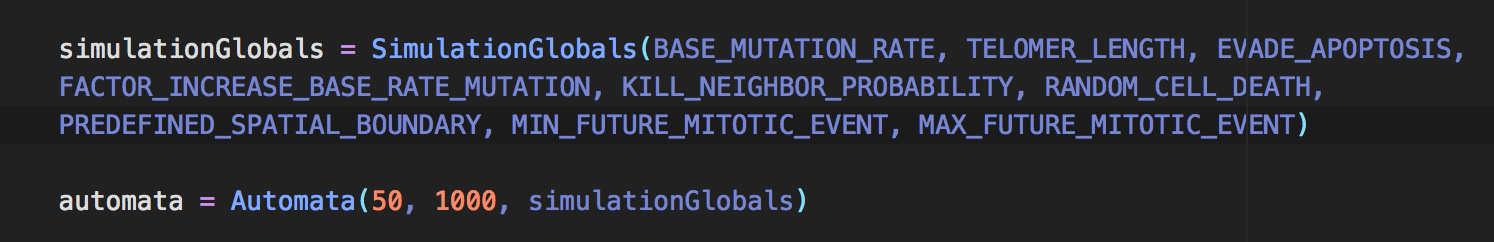
\includegraphics[scale=0.6]{figures/simulations_globals}
\caption{Código para configuración por defecto de una simulación.}
\label{fig:params}
\end{figure}
